% template created by: Russell Haering. arr. Joseph Crop
\documentclass[12pt,letterpaper]{article}
\usepackage{anysize}
\usepackage{graphicx}
\usepackage{enumerate}
\marginsize{2cm}{2cm}{1cm}{1cm}

\usepackage{color}
\usepackage{listings}
\usepackage[utf8]{inputenc}
\usepackage{longtable}

\begin{document}

\begin{titlepage}
    \vspace*{4cm}
    \begin{flushright}
    {\huge
        ECE 375 Homework 2\\[1cm]
    }
    {\large
       Computer Organization and Assembly Language Programming
    }
    \end{flushright}
    \begin{flushleft}
    Winter Term 2018
    \end{flushleft}
    \begin{flushright}
    Jeremy Fischer

    \end{flushright}

\end{titlepage}


\section{Homework Questions}
\begin{enumerate}
    %Question 1
    \item
    Consider the internal structure of the pseudo-CPU discussed in class augmented with a \textit{single-port register file} (i.e., only one register value can be read in a cycle) containing 32 8-bit registers (R0-R31) and a carry bit (Cbit), which is set/reset after each arithmetic operation. 
    Suppose the pseudo-CPU can be used to implement the AVR instruction ADIW ZH:ZL,32 \textit{(Add immediate to word)}. ADIW is a 16-bit instruction, where the upper byte represents the opcode and the lower byte represents an immediate value, i.e., “32” (do not worry about the fact that the actual format is slightly different). 
    Give the sequence of microoperations required to Fetch and Execute the ADIW instruction. 
   \textit{ Your solutions should result in exactly 5 cycles for the fetch cycle and 6 cycles for the execute cycle.} 
    Assume the memory is organized into addressable bytes (i.e., each memory word is a byte), MDR, IR, and AC registers are 8-bit wide, and PC and MAR registers are 16-bit wide. Also, assume Internal Data Bus is 16-bit wide and thus can handle 8-bit or 16-bit (as well as portion of 8-bit or 16-
    bit) transfers in one microoperation and only PC and AC have the capability to increment itself.
   
   	\begin{figure}[h]
   		\centering
   		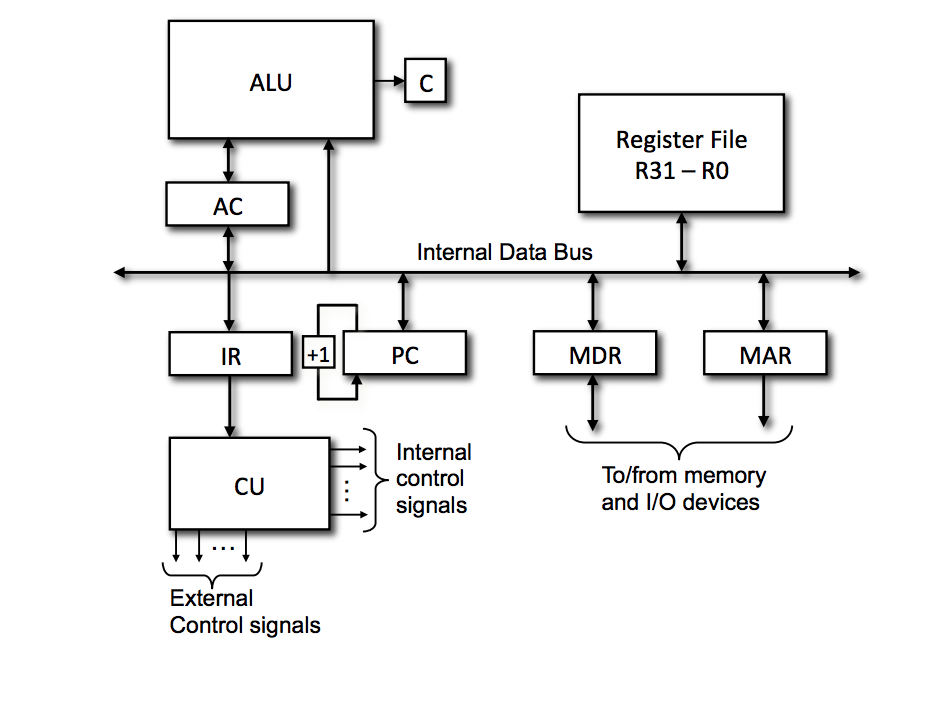
\includegraphics[width=0.6\textwidth]{Q1.png}
   \end{figure}
   
   
   
   \textbf{Answer:}
   
	\begin{center}
		\textit{Fetch Cycle}
	\end{center}

	MAR $\leftarrow$ PC 				\hfill ;load the opcode address
	\\
	MDR $\leftarrow$ M[MAR]; PC $\leftarrow$ PC + 1		\hfill ;load the opcode
	\\
	IR $\leftarrow$ MDR 				\hfill ;load the opcode into IR
	\\
	MAR $\leftarrow$ PC 				\hfill ;load the immediate value address
	\\
	MDR $\leftarrow$ M[MAR]; PC $\leftarrow$ PC + 1 \hfill ;load the immediate value
	
	\begin{center}
		\textit{Execute Cycle}
	\end{center}

	R16 $\leftarrow$ AC \hfill ;store the old value of AC in temp register
	\\
	AC $\leftarrow$ ZL \hfill ;move low byte to AC
	\\
	AC $\leftarrow$ (AC + MDR), ZL $\leftarrow$ AC \hfill ;add low byte and immediate value, move back to ZL
	\\
	AC $\leftarrow$ ZH \hfill ;move high byte to AC
	\\
	AC $\leftarrow$ (AC + C), ZH $\leftarrow$ AC \hfill ;add high byte and carry, move back to ZH
	\\
	AC $\leftarrow$ R16 \hfill ;restore old AC value






	\clearpage
	%Question 2
   \item
   Consider the internal structure of the pseudo-CPU discussed in class augmented with a \textit{single-port register file} (i.e., only one register value can be read at a time) containing 32 8-bit registers (R31-R0) and a Stack Pointer (SP). 
   Suppose the pseudo-CPU can be used to implement the AVR instruction ICALL \textit{(Indirect Call to Subroutine)} with the format shown below: 
   
   \begin{figure}[h]
   		\centering
   		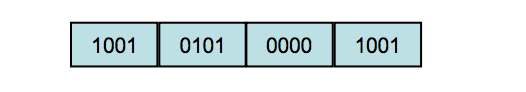
\includegraphics[width=0.45\textwidth]{Q2.png}
   \end{figure}

	ICALL pushes the return address onto the stack and jumps to the 16-bit target address contained in the Z register. 
	Give the sequence of microoperations required to Fetch and Execute AVR’s ICALL instruction.
	\textit{Your solutions should result in exactly 6 cycles for the fetch cycle and 8 cycles for the execute cycle.} 
	Assume the memory is organized into addressable bytes (i.e., each memory word is a byte), MDR is 8 bits, and AC, SP, PC, IR, and MAR are 16 bits. 
	Also, assume Internal Data Bus is 16-bit wide and thus can handle 8-bit or 16-bit (as well as portion of 8-bit or 16-bit) transfers in one microoperation and SP has the capability to increment/decrement itself. 
	Clearly state any other assumptions made.
	\begin{figure}[h]
		\centering
		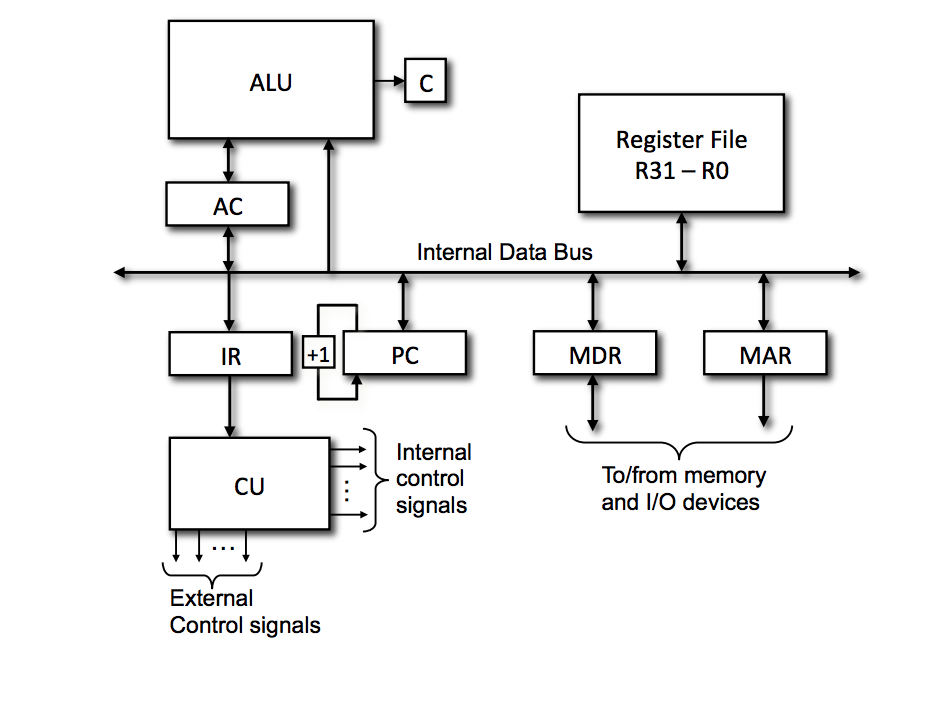
\includegraphics[width=0.55\textwidth]{Q1.png}
	\end{figure}
	 
	 
	\textbf{Answer:}
	
	I am assuming that the program memory is 16-bits wide, and it is possible to access the low and high byte of memory separately.
	
	
	\begin{center}
		\textit{Fetch Cycle}
	\end{center}
		
	
	
	MAR $\leftarrow$ PC\textsubscript{low} 				\hfill ;load the opcode address
	\\
	MDR $\leftarrow$ M[MAR]; 	\hfill ;get the opcode low byte
	\\
	IR\textsubscript{low} $\leftarrow$ MDR 				\hfill ;load the opcode low byte  into IR
	\\
	MAR $\leftarrow$ PC\textsubscript{high}; PC $\leftarrow$ PC + 1					\hfill ;load the opcode address
	\\
	MDR $\leftarrow$ M[MAR];	\hfill  ;get the opcode high byte
	\\
	IR\textsubscript{high} $\leftarrow$ MDR 				\hfill ;load the opcode high byte into IR
	
	\begin{center}
		\textit{Execute Cycle}
	\end{center}
	
	MAR $\leftarrow$ SP\textsubscript{low}	\hfill ;get the low byte address of stack
	\\
	MDR $\leftarrow$ PC\textsubscript{low} \hfill ;get the low byte of return address
	\\
	M[MAR] $\leftarrow$ MDR	\hfill ;load the low byte of ret. to low addr. of stack
	\\
	MAR $\leftarrow$ SP\textsubscript{high} \hfill  ;get the high byte address of stack
	\\
	MDR $\leftarrow$ PC\textsubscript{high} ;SP $\leftarrow$ SP - 1  \hfill ;get the high byte of return address and dec. stack
	\\
	M[MAR] $\leftarrow$ MDR  \hfill ;load the high byte of ret. to high addr. of stack
	\\
	PC\textsubscript{low} $\leftarrow$ ZL \hfill ;load low byte of jump addr. to PC low
	\\
	PC\textsubscript{high} $\leftarrow$ ZH  \hfill ;load high byte of jump addr. to PC high
	
	

	
	
	
	\clearpage
	%Question 3
	\item
	Suppose the following array of numbers are stored in the Data Memory (represented in hexadecimal):
	\begin{figure}[h]
		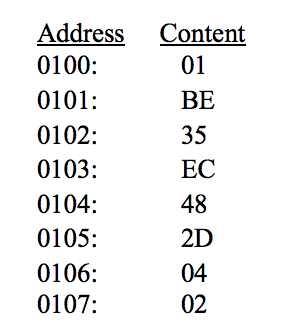
\includegraphics[width=0.3\textwidth]{Q3.png}
	\end{figure}
 	
 	\begin{enumerate}
 		\item 
 		Assuming these numbers are signed numbers, write a subroutine using AVR assembly that (1) determines the smallest number among the 8 numbers stored in memory and (2) stores that number in the memory location \$0108. 
 		Clearly comment and explain your code. 
 		Use the skeleton code shown below to implement your subroutine: 
 		
 		
 		\item
 		Suppose these numbers are unsigned numbers (i.e., they are positive numbers). Show and explain how
 		the code developed in part (a) would have to be modified. 

 		\clearpage
 		
 		\textbf{Answer (a):}
 		
		\textit{I am assuming that "m128def.inc" is included. Therefore, RAMEND = 0x10ff.}
 		
 		\lstinputlisting{Q3.asm}
 		
 		\textbf{Answer (b):}
 		
 		The only thing that would need to be changed is the \textit{BRGE} instruction.
 		BRGE is used for signed numbers.
 		We would change \textit{BRGE} for \textit{BRSH}, since \textit{BRSH} is for unsigned numbers.
 		This would allow the comparisons between numbers (specifically curLow and curV) to function as we expect.
 		
 	\end{enumerate}
		
	\clearpage
	
	%Question 4
	\item
	Determine the location (i.e., address) and binary code for each instruction in the code developed for Problem \#3 part (a). 
	Clearly explain your answers. 
	
	\textbf{Answer:}
	
	\begin{figure}[h]
		\centering
		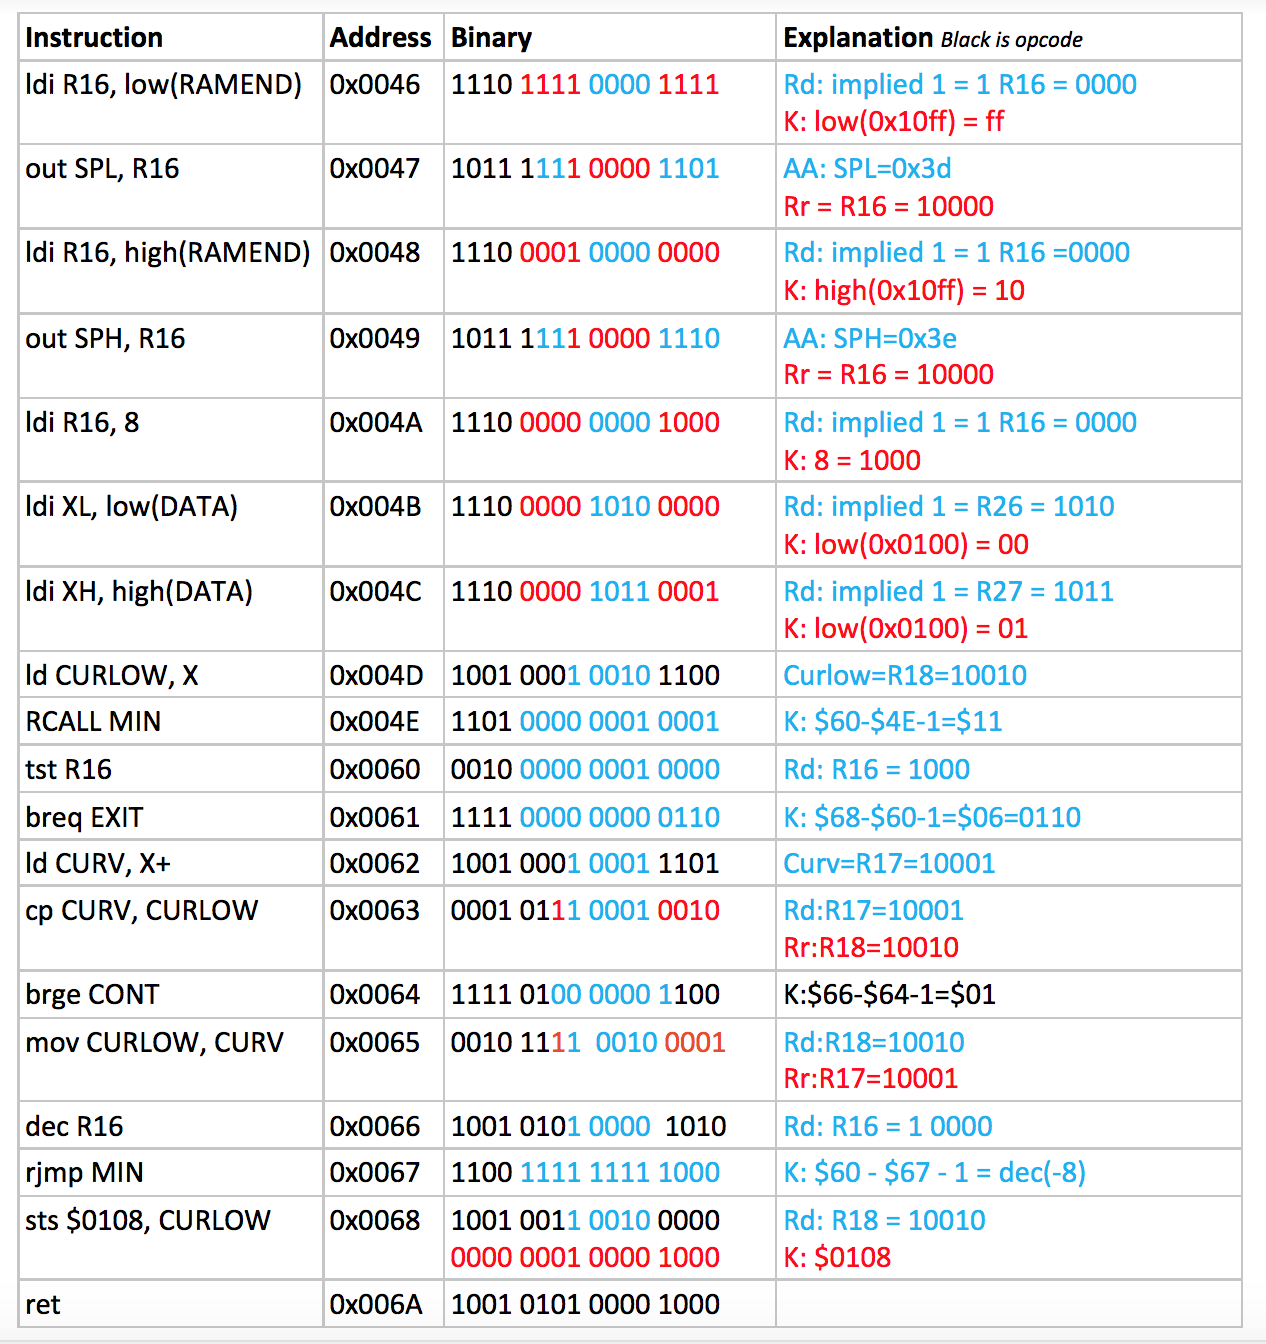
\includegraphics[width=0.9\textwidth]{Q4Answ.png}
	\end{figure}
	
\end{enumerate}


       

\end{document}
